
\documentclass[ms.tex]{subfiles}
\begin{document}

\section{Methods}
\label{sec:methods}

\begin{itemize}

	\item We are interested in applying one-zone GCE models to dwarf galaxies
	and determining best-fit parameters.
	We begin by providing background on one-zone models, and then we select
	a parametrization from which we draw a fiducial mock stellar sample.
	We then use these data to introduce our fitting method.

\end{itemize}

\subsection{One-Zone Models of Galactic Chemical Evolution}
\label{sec:methods:onezone}

\begin{itemize}

	\item The fundamental assumption of one-zone models is that newly produced
	metals mix instantaneously throughout the star forming gas reservoir.
	This approximation is valid as long as the mixing time-scale is negligible
	compared to the depletion time-scale (i.e. the average time an fluid
	element remains in the ISM before getting incorporated into new stars or
	ejected in an outflow).
	Based on the observations of~\citet{Leroy2008},~\citet*{Weinberg2017}
	calculate that characteristic depletion times can range from~$\sim$500 Myr
	up to~$\sim$10 Gyr for conditions in typical star forming disc galaxies.
	With the short length-scales and turbulent velocities of dwarf galaxies,
	instantaneous mixing should be a good approximation.

	\begin{itemize}
		\item {\color{red}
		If there's an observational reference of metal-mixing in the dwarf
		galaxy regime - specifically if the scatter in the~\afe-\feh~plane is
		dominated by observational uncertainty - Evan Kirby would probably be
		the one to know about it.
		If not, this would be a good thing to call out as a good observational
		test of the validity of the one-zone approximation.
		}
	\end{itemize}

	\item The assumption of instantaneous mixing eliminates the need for
	spacial information, reducing GCE to a system of coupled
	integro-differential equations which can be solved numerically.

\end{itemize}

\subsubsection{Inflows, Outflows, Star Formation, and Recycling}
\label{sec:methods:onezone:gas}

\begin{itemize}

	\item At a given moment in time, gas is added to the interstellar medium
	(ISM) via inflows and recycled stellar envelopes and is taken out of the
	ISM via outflows and new stars.
	This gives rise to the following differential equation describing the
	evolution of the gas-supply:
	\begin{equation}
	\label{eq:mdot_gas}
	\dot{M}_\text{g} = \dot{M}_\text{in} - \dot{M}_\star - \dot{M}_\text{out}
	+ \dot{M}_\text{r},
	\end{equation}
	where~$\dot{M}_\text{in}$ is the infall rate,~$\dot{M}_\star$ is the star
	formation rate (SFR),~$\dot{M}_\text{out}$ is the outflow rate,
	and~$\dot{M}_\text{r}$ is the return of stellar envelopes from previous
	generations of stars.

	\begin{itemize}
		\item We relate the SFR to the gas supply by introducing the ``star
		formation efficiency (SFE) timescale'':
		\begin{equation}
		\tau_\star \equiv \frac{M_\text{g}}{\dot{M}_\star},
		\end{equation}
		This quantity is often referred to as the ``depletion time'' in the
		observational literature~\citep[e.g.][]{Tacconi2018}.
		This nomenclature, taken from~\citet{Weinberg2017}, is based on its
		inverse~$\tau_\star^{-1}$ often being referred to as the SFE itself
		because it describes the~\textit{fractional} rate at which some ISM
		fluid element is forming stars.

		\item There are various prescriptions for outflows in the literature.
		Some authors~\citep[e.g.][]{Andrews2017, Weinberg2017} assume a linear
		proportionality between the two:
		\begin{equation}
		\label{eq:eta}
		\dot{M}_\text{out} \equiv \eta\dot{M}_\star.
		\end{equation}
		Recently,~\citet{delosReyes2022} constrained the evolution of the
		Sculptor dwarf spheroidal galaxy with a linear proportionality between
		the SFR and the SN rate~$\dot{N}_\text{II} + \dot{N}_\text{Ia}$.
		\citet*{Kobayashi2020} developed a model in which outflow-driving winds
		develop in the early phases of the Milky Way's evolution, but die out
		on some timescale as the Galaxy grows.
		For modelling the Milky Way, some authors neglect outflows, arguing
		that they do not signicantly alter the chemical evolution of the
		disc~\citep[e.g.][]{Spitoni2019, Spitoni2021}.
		In our mock sample and in our fits to the GSE and the Sagitarrius dSph,
		we assume the linear proportionality given by equation~\refp{eq:eta}.
		Our fitting routine, however, is easily extended to the parametrization
		of~\citet{delosReyes2022}, and if outflows are to be neglected, one can
		simply take~$\eta = 0$ in their fit.

		\item The recycling rate~$\dot{M}_\text{r}$, in general, depends on the
		stellar IMF~\citep[e.g.][]{Salpeter1955, Miller1979, Kroupa2001,
		Chabrier2003}, the initial-final remnant mass relation
		\citep[e.g.][]{Kalirai2008}, and mass-lifetime relation
		(e.g.~\citealp{Larson1974, Maeder1989};~\citealp*{Hurley2000}).
		A single stellar population returns some fraction of its initial
		mass~$r$ back to the ISM according to:
		\begin{equation}
		\label{eq:crf}
		r(\tau) = \ddfrac{
			\int_{m_\text{to}(\tau)}^u (m - m_\text{rem})\frac{dN}{dm} dm
		}{
			\int_l^u m \frac{dN}{dm} dm
		}
		\end{equation}
		where~$l$ and~$u$ are the lower and upper mass limits of star formation,
		respectively,~$m_\text{to}(\tau)$ is the turnoff mass of a stellar
		population of age~$\tau$,~$m_\text{rem}$ is the mass of a remnant left
		behind by a star of initial mass~$m$, and~$dN/dm$ is the adopted IMF.
		Under this prescription, the recycling rate from~\textit{many} stellar
		populations, taking into account the full SFH, is given by:
		\begin{equation}
		\label{eq:mdot_recycled}
		\dot{M}_\text{r} = \int_0^T \dot{M}_\star(t) \dot{r}(T - t) dt
		\end{equation}
		where~$T$ is the time in the model.
		Due to the steep nature of the mass-lifetime relation, the recycling
		rate is dominated by young stellar populations.
		\citet{Weinberg2017} demonstrate that it is sufficiently accurate in
		one-zone models to assume that some fraction~$r_\text{inst}$ of a
		stellar population's initial mass is returned to the ISM immediately
		(see their Fig. 7; they recommend~$r_\text{inst} = 0.4$ for a
		\citealt{Kroupa2001} IMF, and~$r_\text{inst} = 0.2$ for a
		\citealt{Salpeter1955} IMF).
		Although it is simpler to assume~$\dot{M}_\text{r} =
		r_\text{inst}\dot{M}_\star$, numerical integration of equations
		\refp{eq:crf} and~\refp{eq:mdot_recycled} is easy, and~\vice~already
		does it, so we stick with that.

		\item \citet{Weinberg2017} demonstrate that~$\tau_\star$ and~$\eta$
		determine the first-order details of the gas-phase evolutionary track
		in the~\afe-\feh~plane (see their Fig. 2).
		With low~$\tau_\star$ (i.e. high SFE), nucleosynthesis is fast because
		star formation is fast, and a higher metallicity can be obtained before
		the onset of SN Ia than in lower SFE models.
		For this reason,~$\tau_\star$ plays the dominant role in shaping the
		position of the knee in the~\afe-\feh~plane.
		As the galaxy evolves, it approaches a chemical equilibrium in which
		newly produced metals are balanced by the loss of metals to outflows
		and new stars.
		Controlling the strength of the sink term of outflows,~$\eta$ plays
		the dominant role in shaping the late-time equilibrium abundance of the
		model, which high outflow models (i.e. high~$\eta$) predicting lower
		equilibrium abundances than their weak outflow counterparts.
		For observed data, the shape of the track itself directly constrains
		these parameters.
		The detailed form of the SFH has minimal impact on the shape of the
		tracks; rather, that information is encoded in the density of points
		along the evolutionary track and in the stellar metallicity
		distribution functions (MDFs).

	\end{itemize}

\end{itemize}

\subsubsection{Core Collapse Supernovae}
\label{sec:methods:onezone:ccsne}

\begin{itemize}

	\item Massive stars, their winds, and their supernovae enrich the ISM on
	short timescales due to their short lifetimes.
	As long as the relevant timescales for galaxy evolution are significantly
	longer than the lifetimes of massive stars, it is adequate to approximate
	this nucleosynthetic material as ejected instantaneously following a single
	stellar population's formation.
	This implies a linear relationship between the CCSN enrichment rate and
	the SFR:
	\begin{equation}
	\label{eq:mdot_cc}
	\dot{M}_\text{x}^\text{CC} = y_\text{x}^\text{CC}\dot{M}_\star
	\end{equation}
	where~$y_\text{x}^\text{CC}$ is the IMF-averaged fractional net yield from
	massive stars.
	In parameterizing this term with an IMF-averaged yield, we ipmlicitly assume
	that the stellar mass is sufficiently high such that stochastic sampling of
	the IMF is an insignificant effect.

\end{itemize}

\subsubsection{Type Ia Supernovae}
\label{sec:methods:onezone:sneia}

\begin{itemize}

	\item Unlike CCSN enrichment, SN Ia enrichment can occur on delay
	timescales of a Gyr or more.
	In general, the enrichment rate can be expressed as an integral over the
	SFH weighted by the delay-time distribution (DTD):
	\begin{equation}
	\dot{M}_\text{x}^\text{Ia} = y_\text{x}^\text{Ia} \ddfrac{
		\int_0^{T - t_\text{D}} \dot{M}_\star(t) R_\text{Ia}(T - t) dt
	}{
		\int_0^\infty R_\text{Ia}(t) dt
	},
	\end{equation}
	where~$R_\text{Ia}(t)$ is the DTD itself.
	By comparing the cosmic SFH~\citep[e.g.][]{Madau2014} with the cosmic SN
	Ia rate, the cosmic SN Ia DTD appears consistent with a uniform~$t^{-1}$
	power-law (e.g.~\citealp{Maoz2012a};~\citealp*{Maoz2012b, Graur2013}).
	Following~\citet{Weinberg2017}, we take a~$t^{-1.1}$ power-law DTD with a
	minimum delay-time of~$t_\text{D} = 150$ Myr.

	\item In general, the mass of some element x in the ISM is also affected by
	outflows, recycling, star formation, and infall.
	The enrichment rate can be calculated by simply adding up all of the source
	terms and subtracting the sink terms:
	\begin{equation}
	\label{eq:enrichment_eq}
	\dot{M}_\text{x} = \dot{M}_\text{x}^\text{CC} + \dot{M}_\text{x}^\text{Ia}
	- Z_\text{x}\dot{M}_\star - Z_\text{x}\dot{M}_\text{out} +
	\dot{M}_\text{x,r},
	\end{equation}
	where the rate of return of the element x from recycled stellar envelopes
	can be computed by weighting the integral in equation~\refp{eq:mdot_recycled}
	by~$Z_\text{x}(t)$.
	If there is metal-rich infall, this equation picks up the additional term
	$Z_\text{x,in}\dot{M}_\text{in}$ quantifying that, although here we assume
	that infall is pristine.

\end{itemize}

\subsubsection{Nucleosynthetic Yields}
\label{sec:methods:onezone:yields}

\begin{itemize}

	\item In general, nucleosynthetic yields are degenerate with the outflow
	mass loading factor~$\eta$.
	We quantify this is in more detail in Appendix X, simply noting there that
	the two are simply the dominant source and sink terms, and as such,
	high-yield high-outflow models generally have a low-yield low-outflow
	counterpart that predicts a similar chemical evolution.
	In order to break this degeneracy, only one number setting the absolute
	scale is required.
	Here, we simply set the alpha element yield to~\yacc~= 0.01.
	This value is somewhat informed by nucleosynthesis theory in that
	massive star evolutionary models (e.g.~\citealp{Sukhbold2016,
	Limongi2018};~\citealp*{Nomoto2013}) typically predict
	$y_\text{O}^\text{CC} = 0.005 - 0.015$ (see discussion in, e.g.,
	\citealp{Weinberg2017, Johnson2020}), but is otherwise intended to be a
	round number from which our best-fit values affected by this degeneracy can
	simply be scaled up or down.

	\item We let our Fe yields~\yfecc~and~\yfeia~be free parameters.
	With this approach, we implicitly fit the height of the [$\alpha$/Fe]
	plateau as well as the Fe yield ratio~\yfecc/\yfeia.

	\item In general, nucleosynthetic material is also expelled by asymptotic
	giant branch (AGB) stars~\citep[e.g.][]{Cristallo2011, Cristallo2015,
	Ventura2013, Karakas2016, Karakas2018}.
	Here we are interested primarily in~$\alpha$ and Fe-peak elements, elements
	whose AGB star yields are negligible compared to their SN yields
	\citep[e.g.][]{Johnson2019}.
	We therefore omit discussion of AGB star nucleosynthesis here, but we note
	that our fitting method described in~\S~\ref{sec:methods:fitting} is easily
	extensible to include an AGB star enrichment channel.
	Mathematical details of how this is implemented in~\vice~can be found in
	\citet{Johnson2020},~\citet{Johnson2022}, and in the~\vice~science
	documentation.\footnote{
		\url{https://vice-astro.readthedocs.io/en/latest/science_documentation/index.html}
	}

\end{itemize}

\subsection{A Fiducial Mock Sample}
\label{sec:methods:fiducialmock}

\begin{figure*}
\centering
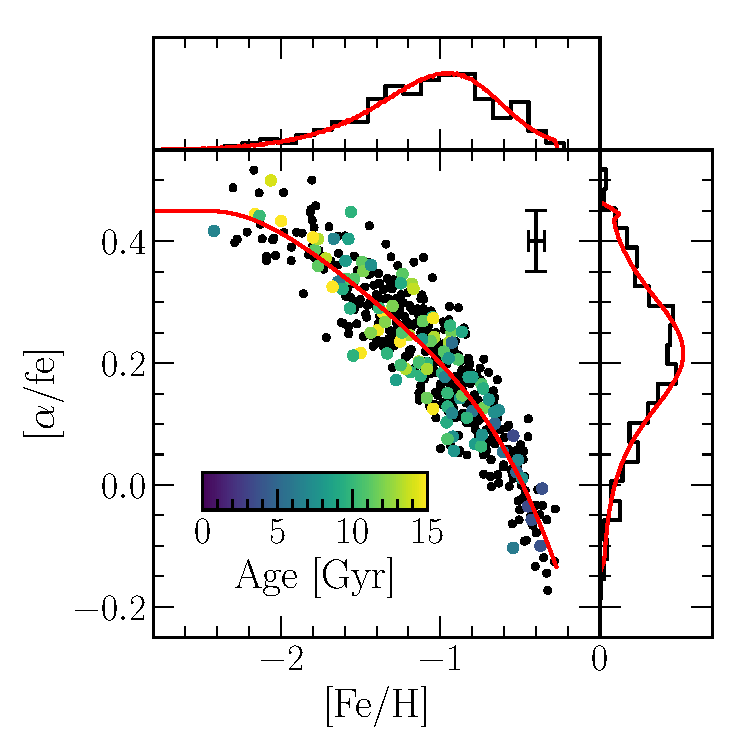
\includegraphics[scale = 0.5]{fiducial_mock_afe_feh.pdf}
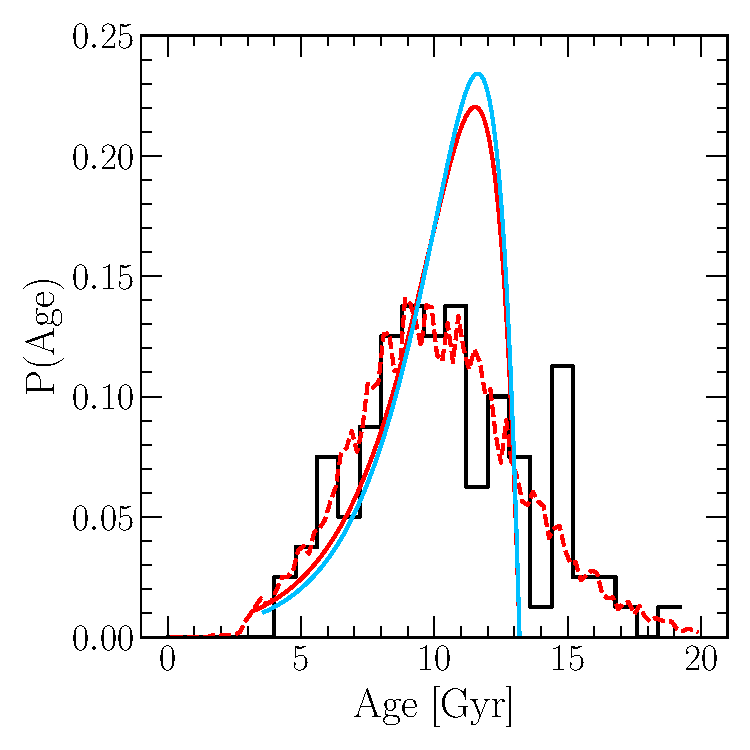
\includegraphics[scale = 0.42]{fiducial_mock_agedist.pdf}
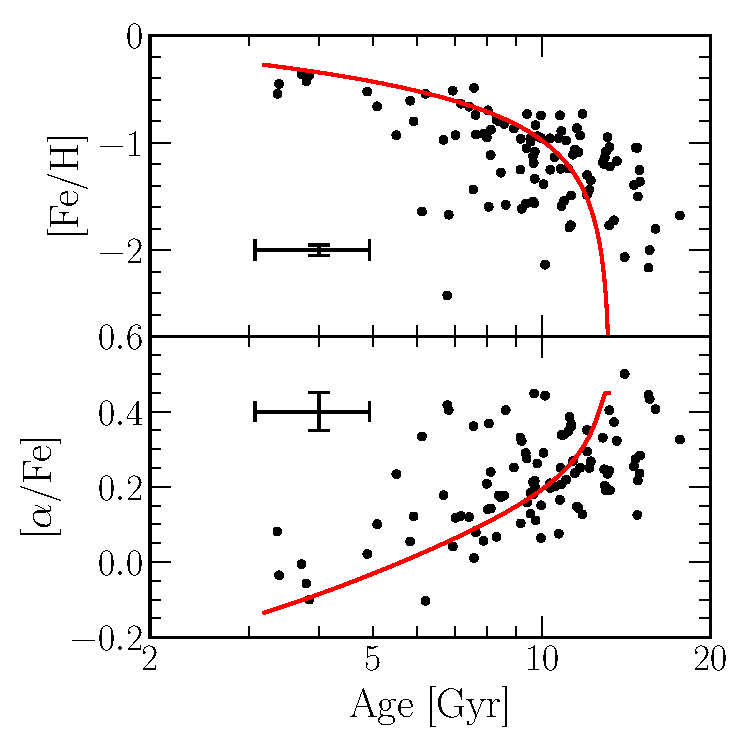
\includegraphics[scale = 0.42]{fiducial_mock_amr.pdf}
\caption{
\textbf{Left}: Our fiducial mock sample in the~\afe-\feh~plane.
There are~$N = 500$ stars with abundance uncertainties
of~$\sigma(\feh) = \sigma(\afe) = 0.05$ as indicated by the errorbar.
$N = 100$ of the stars have age information available with an artificial
uncertainty of~$\sigma(\log_{10}(\text{age})) = 0.1$ as indicated by the
colorbar.
The red line denotes the evolutionary track in the gas-phase from the one-zone
model that generated the mock.
On the top and right, we show the marginalized distributions
in~\afe~and~\feh, with red lines denoting the known distribution.
\textbf{Center}: The mock (black, binned) and known (red) age distributions.
The dashed red line indicates the age distribution that is obtained by sampling
$N = 10^4$ rather than $N = 500$ stars and assuming the same age uncertainty
of~$\sigma(\log_{10}(\text{age})) = 0.1$.
\textbf{Right}: The age-\feh~(top) and age-\afe~(bottom) relation for the mock
sample, with artificial uncertainties denoted by the error bars on each panel.
The red lines denotes the known relations for the gas-phase.
}
\label{fig:fiducialmock}
\end{figure*}

\begin{table}
\caption{
The known parameters of the one-zone model from which we generate our mock
stellar samples.
}
\begin{tabularx}{\columnwidth}{l @{\extracolsep{\fill}} l r}
\hline
Parameter & Description & Value
\\
\hline
$\tau_\text{in}$ & e-folding timescale of the infall history & 2 Gyr
\\
$\eta$ & Outflow mass-loading factor
($\eta \equiv \dot{M}_\text{out} / \dot{M}_\star$) & 10
\\
$\tau_\star$ & SFE timescale ($\tau_\star \equiv M_\text{g} / \dot{M}_\star$) &
15 Gyr
\\
$\tau_\text{tot}$ & Duration of star formation & 10 Gyr
\\
\yfecc & IMF-averaged fractional net Fe yield from CCSNe & 0.0008
\\
\yfeia & IMF-averaged fractional net Fe yield from SN Ia & 0.0011
\\
\hline
\end{tabularx}
\end{table}

\begin{itemize}

	\item We use our parametrization of one-zone GCE models described
	in~\S~\ref{sec:methods:onezone} to set up an underlying model from which
	mock samples can be drawn; we then use a fiducial mock sample to describe
	our fitting method in~\S~\ref{sec:methods:fitting} and explore variations
	in, e.g., sample size and precision.

	\item We take an exponential infall history described by
	\begin{equation}
	\dot{M}_\text{in} \propto e^{-t/\tau_\text{in}}
	\end{equation}
	with~$\tau_\text{in} = 2$ Gyr and an initial gas mass of 0.
	The overall normalization of the infall history is irrelevant because
	mass information cancels in one-zone models when you compute abundances.
	We additionally select~$\tau_\star = 15$ Gyr and~$\eta = 10$ with the
	thought that slow star formation and strong outflows would mimic the
	evolution seen in a typical field dwarf galaxy.
	We set the onset of star formation~$\tau = 13.2$ Gyr ago, allowing~$\sim$0.5
	Gyr between the Big Bang and the first stars.
	We evolve this model for 10 Gyr (i.e. the exact ages of the youngest stars
	in the mock sample are~$\tau = 3.2$ Gyr).

	\item {\color{red} YIELDS}

	\item One-zone models produce stellar populations rather than individual
	stars, so if a mock sample of individual stars is to be obtained, we must
	sample from the underlying population.
	Higher mass stellar populations have proportionally more stars than lower
	mass stellar populations, so we take the probability of sampling to be
	proportional to the mass of a population.
	In the interest of mimicing typical observational samples for local group
	dwarfs, we take~$N = 500$ stars with abundance uncertainties of
	$\sigma\afe = \sigma\feh = 0.05$.
	100 of these stars have age information with an uncertainty
	of~$\sigma\logage = 0.1$.

	\item We illustrate this sample in Fig.~\ref{fig:fiducialmock}.
	This sample shows a ``knee'' in the~\afe-\feh~diagram near~\feh~$\sim$-2.3
	and an equilibrium abundance near~\feh~$\sim$-0.3, but due to the
	declining nature of the SFH, most of the stars form in
	the~\feh~$\sim$-1 and~\afe~$\sim$+0.2 region of chemical space.

\end{itemize}


\subsection{The Fitting Method}
\label{sec:methods:fitting}

\begin{itemize}

	\item Here we present our method for applying one-zone GCE models to a
	series of observed abundances and determining the best-fit values.
	The generic statistical problem at play here is the~\textit{inhomogeneous
	poisson point process} (IPPP).
	By applying the principles of an IPPP to models which produces tracks in
	some observed space, we can infer the best-fit parameters given some set
	of noisy observables in that space.
	Such models arise not only in the context of chemical evolution as in this
	work, but also in stellar streams and color-magnitude diagrams (i.e.
	stellar isochrones).
	This approach should therefore be extensible to these topics as well.

	% \item In this section, we present our method for applying one-zone GCE
	% models to a series of points in the~\afe-\feh~plane and determining the
	% best-fit values of the parameters.
	% The more generic statistical problem at play here is to infer the parameters
	% of models which produce tracks in some observed space from a set of noisy
	% observations of individuals in that space.
	% Such models arise not only in the context of chemical evolution as in this
	% work, but also in stellar streams and color-magnitude diagrams (i.e. stellar
	% isochrones); this approach should therefore be extensible to these topics.

	\item Our approach makes the following assumptions regarding the track and
	the data:
	\begin{itemize}

		\item[\textbf{1.}] The track is infinitely thin. In the absence of
		observational errors, all of the data would fall perfectly on a line
		in~$J$-dimensional space.

		\item[\textbf{2.}] The density~\textit{along} the track changes slowly
		relative to the observational uncertainties.

		\item[\textbf{3.}] The observational uncertainties on the data are
		described by a multivariate Gaussian.

		\item[\textbf{4.}] All of the data are associated with the model.

		\item[\textbf{5.}] The sample selection is not a function of the
		observables (though this can be relaxed; see discussion on weights
		below).

	\end{itemize}

	\item For a given data sample~\script{D}, the goal is to find the
	model~\script{M} predicted by a set of parameters~$\theta$ which maximizes
	the~\textit{posterior probability}~$L(\script{M} | \script{D})$.
	In practice, however, best-fit values for~$\theta$ are obtained by
	maximizing the~\textit{likelihood function}~$L(\script{D} | \script{M})$
	describing the probability of observing the data~\script{D} given the
	model~\script{M}.
	Bayes' Theorem relates the two according to:
	\begin{equation}
	\label{eq:bayes_theorem}
	L(\script{M} | \script{D}) = \frac{
		L(\script{D} | \script{M}) L(\script{M})
	}{
		L(\script{D})
	}
	\end{equation}
	where~$L(\script{M})$ is the likelihood of the model (known as
	the~\textit{prior}) and~$L(\script{D})$ is the likelihood of the data
	(known as the~\textit{evidence}).
	The evidence is an overall constant of normalization, but the prior can
	influence the best-fit values determined by folding in any existing
	information on the model parameters.
	In general, it is common to assume a ``flat'' (or ``uniform'') prior when
	no additional information is available, and therefore
	$L(\script{M} | \script{D}) \approx L(\script{D} | \script{M})$.

	\item In this context, the goal is to combine the likelihoods for~$N$
	discrete observations and compute a single likelihood for a given track.
	As long as each datum is independent of the rest of the sample, the total
	likelihood can be expressed as the product of the likelihood of each
	individual datum~$\script{D}_i$:
	\begin{subequations}\begin{align}
	L(\script{D} | \script{M}) &= \prod_i L(\script{D}_i | \script{M})
	\\
	\implies \ln L(\script{D} | \script{M}) &= \sum_i \ln L(\script{D}_i |
	\script{M})
	\label{eq:l_d_m}
	\end{align}\end{subequations}

	\item Computing the likelihood of observing the datum~$\script{D}_i$ given
	some model~$M$ is non-trivial because~$\script{D}_i$ came from an unknown
	location along the track.
	We therefore marginalize~$L(\script{D}_i | M)$ over the entirety
	of~\script{M} by integrating the likelihood of a particular observed data
	point along the entire track.
	In practice, models will sample the track at some set of~$K$ points
	$\script{M} = \{\script{M}_1, \script{M}_2, \script{M}_3, ... , 
	\script{M}_K\}$, allowing the~$L(\script{D}_i | \script{M})$ to be
	expressed as a summation over all model points~$\script{M}_j$:
	\begin{equation}
	\label{eq:l_di_m}
	L(\script{D}_i | \script{M}) = \sum_j L(\script{D}_i | \script{M}_j).
	\end{equation}
	There are two important factors which additionally influence
	$L(\script{D}_i | \script{M}_j)$:
	\begin{itemize}

		\item[\textbf{1.}] The inherent density of objects at the
		point~$\script{M}_j$.
		In the context of chemical evolution, this is directly related to the
		star formation rate.
		If the SFR is high at a time~$j$, then it is proprtionally more likely
		that the datum~$\script{D}_i$ is associated with the model point
		$\script{M}_j$ than at another point in time when the SFR is lower.
		In the context of, e.g., stellar isochrones and color-magnitude
		diagrams, this is related to the IMF.

		\item[\textbf{2.}] The selection function of the sample at the
		point~$\script{M}_j$.
		If the survey design is such that different regions of the track are
		sampled more deeply than others, this will be reflected in the
		distribution in the observed space.
		In the context of chemical evolution, this can happen by proxy of
		selection choices in, e.g., stellar age, luminosity, or color.

	\end{itemize}

	Because of these factors directly influencing the likelihood function, it
	is crucial to introduce weights which scale as the product of these two
	effects:
	\begin{equation}
	\label{eq:weights}
	w_j \propto \script{S}(\script{M}_j) \dot{M}_{\star,j}
	\end{equation}
	where~$\script{S}(\script{M}_j)$ is the selection function of the sample
	at the point~$\script{M}_j$ along the track and~$\dot{M}_{\star,j}$ is the
	model-predicted SFR at time~$j$.

	\item If the uncertainties of the datum~$\script{D}_i$ are adequately
	described by a multivariate Gaussian, then with the proper weighting,
	$L(\script{D}_i | \script{M}_j)$ can be expressed as a classical
	$L \propto e^{-\chi^2 / 2}$ expression:
	\begin{equation}
	\label{eq:chi_squared}
	\chi^2 = \Delta_{ij} C_i^{-1} \Delta_{ij}^T
	\end{equation}
	where~$C_i^{-1}$ is the inverse covariance matrix associated with the datum
	$\script{D}_i$ and~$\Delta_{ij} = \script{D}_i - \script{M}_j$ is the
	vector difference between the datum and a given point along the track.

	\item Combining equations~\refp{eq:l_d_m},~\refp{eq:l_di_m},
	\refp{eq:weights}, and~\refp{eq:chi_squared} results in the following
	expression for the likelihood function of the data~\script{D} given the
	track~\script{M}:
	\begin{equation}
	\label{eq:likelihood_func}
	\ln L(\script{D} | \script{M}) = \sum_i \ln \left(
	\sum_j w_j \exp\left(\frac{-1}{2}\Delta_{ij} C_i^{-1} \Delta_{ij}^T\right)
	\right),
	\end{equation}
	where the summations are taken over the entirety of the track and the
	entirety of the data.

	\item In detail, an IPPP requires the sum of the weights~$\sum_j w_j$ to be
	subtracted from~$\ln L(\script{D} | \script{M})$.
	The purpose of this term is such that tracks which go ``too far'' in the
	observed space are penalized for predicting data in regions where there are
	none.
	However, in the context of chemical evolution, the weights are derived from
	the SFH of the model.
	For the models we consider here, the normalization of the SFH is
	inconsequential to the model predictions (i.e. a model with the SFH
	amplified by~$10^6$ at all times but otherwise the same evolutionary
	parameters would predict the same evolution in~\feh~and~\afe).
	For this reason, it is essential that~$\sum_j w_j$ not impact the inferred
	value of~$\ln L(\script{D} | \script{M})$.
	We therefore set~$\sum_j w_j = 1$ always, and tracks which extend too far
	in chemical space are penalized by contributing a~\textit{fractional}
	weight far from the observed points, thereby increasing~$\chi^2$.
	However, for applications of this method in which the sum of the weights
	is~\textit{not} inconsequential to the likelihood function, this additional
	term in equation~\refp{eq:likelihood_func} must be included.
	{\color{red}(It may be worthwhile to include an appendix in which we
	demonstrate the validity of this approach)}.

	\item Although there are variety of ways in which one could construct the
	likelihood function~$L(\script{D} | \script{M})$, in the present paper we
	use the Markov Chain Monte Carlo (MCMC) method.
	Despite being more computationally expensive than, e.g., maximum likelihood
	estimates, MCMC methods offer a more generic solution than by sampling
	tails and multiple modes of the likelihood distribution that would
	otherwise be missed by assuming Gaussianity.
	With this choice, this method should be applicable to additional data sets
	perhaps described by GCE models with different parametrizations.

	\item We use the~\mc~software~\citep{Foreman-Mackey2013} to run our MCMC
	fits.
	At each step in parameter space,~\mc~makes a call to~\vice~to compute the
	predicted abundances for that selection of parameters.
	We then compute the likelihood function~$L(\script{D} | \script{M})$
	according to equation~\refp{eq:likelihood_func} and let~\mc~take care of
	the rest.

	\item In~\S~\ref{sec:methods:mocksamplefits}, we apply this method to our
	fiducial mock sample and discuss how the accuracy and precision of the
	recovered known parameters is affected by sample size, precision, and
	the availability of age information.

\subsection{Mock Sample Fits}
\label{sec:methods:mocksamplefits}

\end{itemize}

\end{document}
